\documentclass{clbeamer2024}

\usepackage{minted}

\usepackage{minted}
\setminted{
	breaklines=true,
	frame=single,
	bgcolor=lightgray,
	fontsize=\small,
	escapeinside=||
}

\usepackage{xcolor}
\definecolor{bg}{rgb}{0.95, 0.95, 0.92} % Couleur gris clair

\title{
	%
\includegraphics[width=0.5cm]{logos/IA1.png} \hfill
        Introduction à Node.js
	
\includegraphics[width=0.7cm]{logos/node.png} \hfill
}
\subtitle{Comprendre les bases du développement serveur avec JavaScript}
\author{Slimani Mohamed Amine}
\institute{EHTP}
\date{\today}

\begin{document}
	\setcounter{framenumber}{-1}
	\frame{\titlepage}
	
	
	
	% Sommaire
	\begin{frame}{Sommaire}
		\tableofcontents
	\end{frame}
	
	\section{Qu'est-ce que Node.js ?}
	\begin{frame}{Qu'est-ce que Node.js ?}
		\begin{itemize}
			\item \textbf{Définition} : Node.js est une plateforme JavaScript côté serveur basée sur le moteur V8 de Chrome.
			\item \textbf{Objectif} : Permettre de créer des applications web rapides et scalables.
			\item \textbf{Avantages} : Modèle non bloquant (asynchrone), grande communauté, riche écosystème de modules.
		\end{itemize}
	\end{frame}
	
	
	\section{Pourquoi utiliser Node.js ?}
	\begin{frame}{Pourquoi utiliser Node.js ?}
		\begin{itemize}
			\item \textbf{Performance} : Modèle non bloquant pour des applications rapides.
			\item \textbf{Scalabilité} : Facile à scaler horizontalement et verticalement.
			\item \textbf{JavaScript partout} : Utiliser le même langage côté client et serveur.
		\end{itemize}
	\end{frame}
	
	
	\section{Composants de Node.js}
	\begin{frame}{Composants de Node.js}
		\begin{itemize}
			\item \textbf{Moteur V8} : Exécute le code JavaScript.
			\item \textbf{Libuv} : Bibliothèque pour la gestion des entrées/sorties asynchrones.
			\item \textbf{NPM (Node Package Manager)} : Gestionnaire de packages pour Node.js.
		\end{itemize}
	\end{frame}
	
	\section{Architecture de Node.js}
	\begin{frame}{Architecture de Node.js}
		\begin{itemize}
			\item \textbf{Boucle d'événements (Event Loop)} : Gère les opérations asynchrones.
			\item \textbf{Thread Pool} : Exécute les tâches bloquantes en parallèle.
			\item \textbf{Modules natifs} : Fournit des fonctionnalités de base (ex : `http`, `fs`).
		\end{itemize}
	\end{frame}
	
	
	\section{Exemple de code Node.js}
	\begin{frame}{Exemple de code Node.js}
		
		\begin{exampleblock}{Serveur HTTP simple}
			
			\begin{center}
			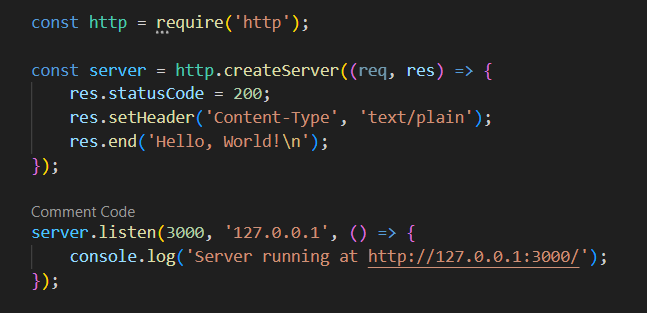
\includegraphics[width=0.87\textwidth]{images/code1.png}
		\end{center}
			
		\end{exampleblock}
		
	\end{frame}
	
	
	\section{Bonnes pratiques}
	\begin{frame}{Bonnes pratiques}
		\begin{itemize}
			\item \textbf{Utiliser des modules} : Diviser le code en modules réutilisables.
			\item \textbf{Gestion des erreurs} : Utiliser des middlewares pour capturer les erreurs.
			\item \textbf{Optimisation des performances} : Utiliser des techniques de caching et de compression.
		\end{itemize}
	\end{frame}
	
	
	\section{Outils pour travailler avec Node.js}
	\begin{frame}{Outils pour travailler avec Node.js}
		\begin{itemize}
			\item \textbf{Express.js} : Framework web pour Node.js.
			\item \textbf{Socket.IO} : Bibliothèque pour les applications en temps réel.
			\item \textbf{PM2} : Gestionnaire de processus pour Node.js.
		\end{itemize}
	\end{frame}
	
	\section{Exemple d'application avec Express.js}
	\begin{frame}{Exemple d'application avec Express.js}
		\begin{exampleblock}{Application web simple}
				\begin{center}
				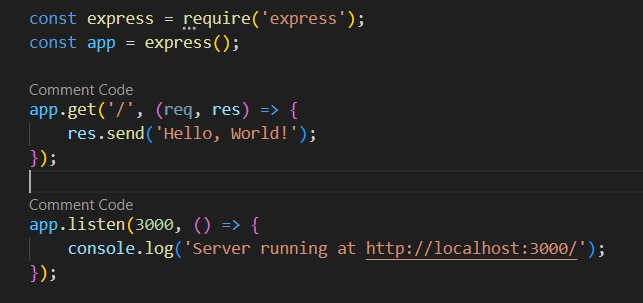
\includegraphics[width=0.87\textwidth]{images/code2.png}
			\end{center}
		
		\end{exampleblock}
	\end{frame}
	
	
	\section{Défis de Node.js}
	\begin{frame}{Défis de Node.js}
		\begin{itemize}
			\item \textbf{Gestion des erreurs} : Les erreurs non capturées peuvent faire planter l'application.
			\item \textbf{Performance CPU-intensive} : Node.js n'est pas idéal pour les tâches gourmandes en CPU.
			\item \textbf{Compatibilité} : Certains modules ne sont pas compatibles avec les dernières versions de Node.js.
		\end{itemize}
	\end{frame}
	
	\section{Pourquoi c'est important ?}
	\begin{frame}{Pourquoi c'est important ?}
		\begin{itemize}
			\item Node.js est une plateforme puissante pour créer des applications web rapides et scalables.
			\item Il permet d'utiliser JavaScript côté serveur, ce qui simplifie le développement full-stack.
			\item Comprendre Node.js est essentiel pour les développeurs web et les architectes logiciels.
		\end{itemize}
	\end{frame}
	
	
	\begin{frame}{Résumé}
		\textbf{Node.js} est une plateforme révolutionnaire pour le développement d'applications serveur rapides et scalables.  
		Développez mieux, plus vite, et avec JavaScript partout !
	\end{frame}
	
	
	
	
	
	
	
\end{document}
